\section{Суралцах явцын дашбоард}

Энэхүү дашбоардыг дадлагын төлөвлөгөөний суралцах эхний 4-н долоо хоногт долоо долоон хоногоор суралцсан зүйлсээ ашиглан сайжруулан хийсэн.

Сурах ур чадвар: 
\begin{itemize}
    \item Tableau-ийн анхан болон ахисан түвшиний зүйлсийг суралцах
    \item Дашбоард өрөхөд шаардлагатай чадваруудыг суралцах
\end{itemize}

Дашбоардыг хийхдээ анхандаа өгөгдлөө бэлдэх буюу 1212.mn-ээс нээлттэй Монгол улсын хүн амын тоо, дундаж цалингийн тоон мэдээлэл, ДНБ-ы хэмжээ зэргийн статистик мэдээллийг хүснэгт хэлбэрээр аван өгөгдлөө цэвэрлэх, зөв бүтэцтэй болгон засварчилсан. Түүний дараа алхам алхамуудаар table-ийн ойлголт, хэрэглүүрүүдийг суралцан дашбоардаа хийгдсэн.

Дашбоард: \url{https://public.tableau.com/app/profile/adiya.hella/viz/_16880920782180/Story1}
\begin{figure}
	\centering
	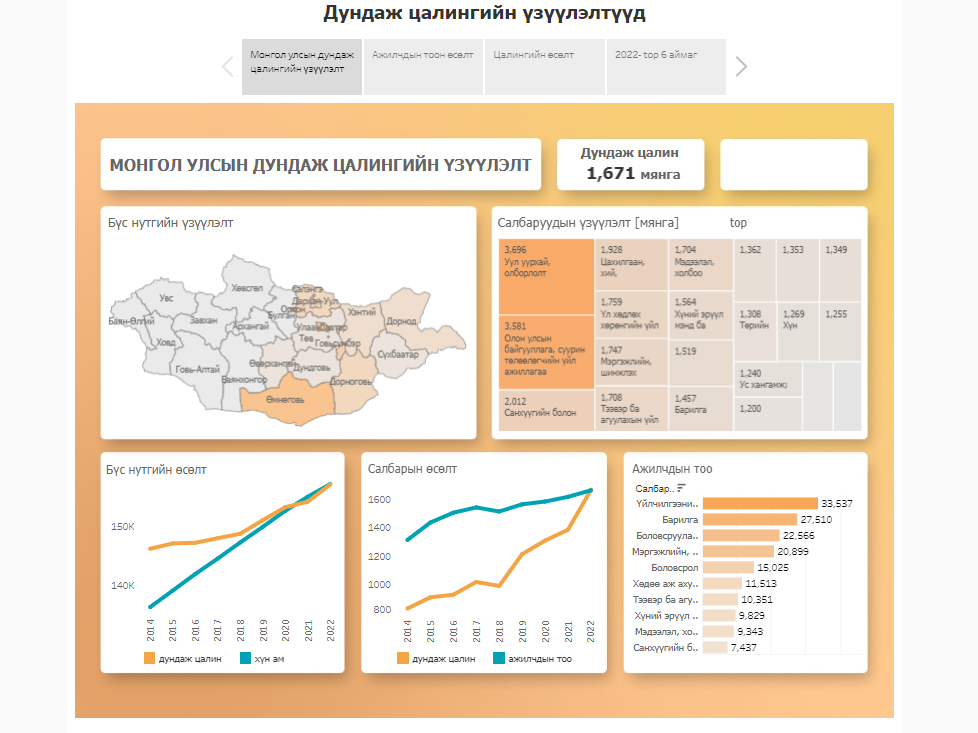
\includegraphics[width=15cm]{images/dash1.PNG}
	\caption{Суралцах явцын дашбоард}
	\label{fig:form}
\end{figure}

\newpage
\section{Төслийн багт оролцон гүйцэтгэсэн ажил}

Энэхүү дашбоардыг өмнө хийсэн байсан дашбоард нь хэрэглэгч буюу захиалагчийн үнэлэмжинд хүрээгүй тул хамт дадлагын хөтөлбөрт хамрагдсан оюутантай хамтран эхнээс нь хэрэглэгчийн шаардлагад нийцүүлэн гүйцэтгэсэн.

\subsection{Ажилыг гүйцэтгэсэн алхамууд}

% \begin{itemize}
%     \item Өгөгдлийн сантай танилцаж, хэрхэн хоорондоо хамааралтай байгаа зэргийг ойлгон мөн хэрэглэгч ямар ямар мэдээллийг харуулахыг хүсэж буй мэдээлэлтэй танилцсан. 
	
% 	\centering
% 	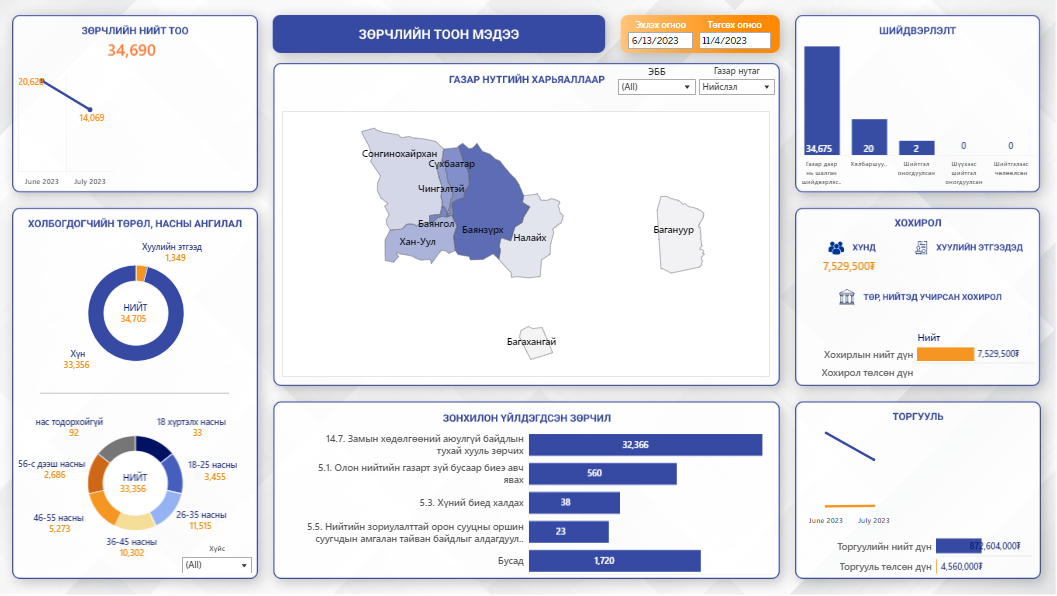
\includegraphics[width=15cm]{images/dash2.PNG}
% 	\item Дашбоард өрөхөд шаардлагатай чадваруудыг суралцах
% \end{itemize}
\begin{itemize}
	\item Өгөгдлийн сантай танилцаж, хэрхэн хоорондоо хамааралтай байгаа зэргийг ойлгон мөн хэрэглэгч ямар ямар мэдээллийг харуулахыг хүсэж буй мэдээлэлтэй танилцсан. 
	\item \begin{minipage}[t]{\linewidth}
			  \centering
			  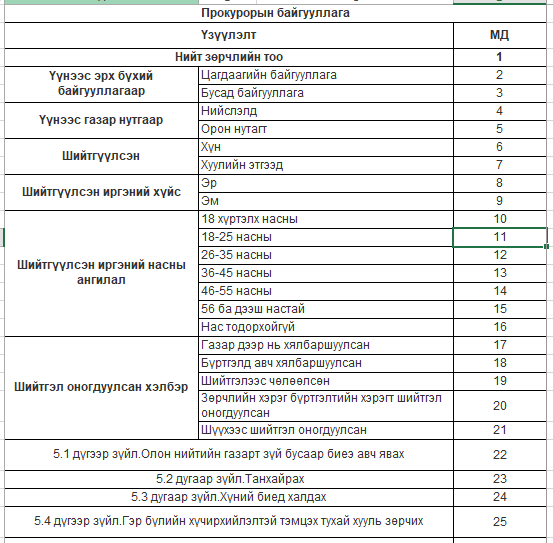
\includegraphics[width=8cm,height=10cm]{images/harahzuils.PNG}
			  \captionof{figure}{Харуулах шаардлагатай мэдээллийн жагсаалт}
		  \end{minipage}
	\item Жагсаалттай танилцсаны дараа хэрхэн ямар ямар графикаар харуулахыг тодорхойлон гракуудыг tableau дээр өрсөн.
	\item Дашбоардын загварыг гаргахдаа өрсөн графикынхаа ард зураг хэлбэрээр харуулах боломжтой байдаг учраас Figma дээр Grid хуваалт ашиглан хэрэглэгчийн нүдэнд таатай, үзэмжтэй байхаар загварчилсан.
	\item \begin{minipage}[t]{\linewidth}
				\centering
				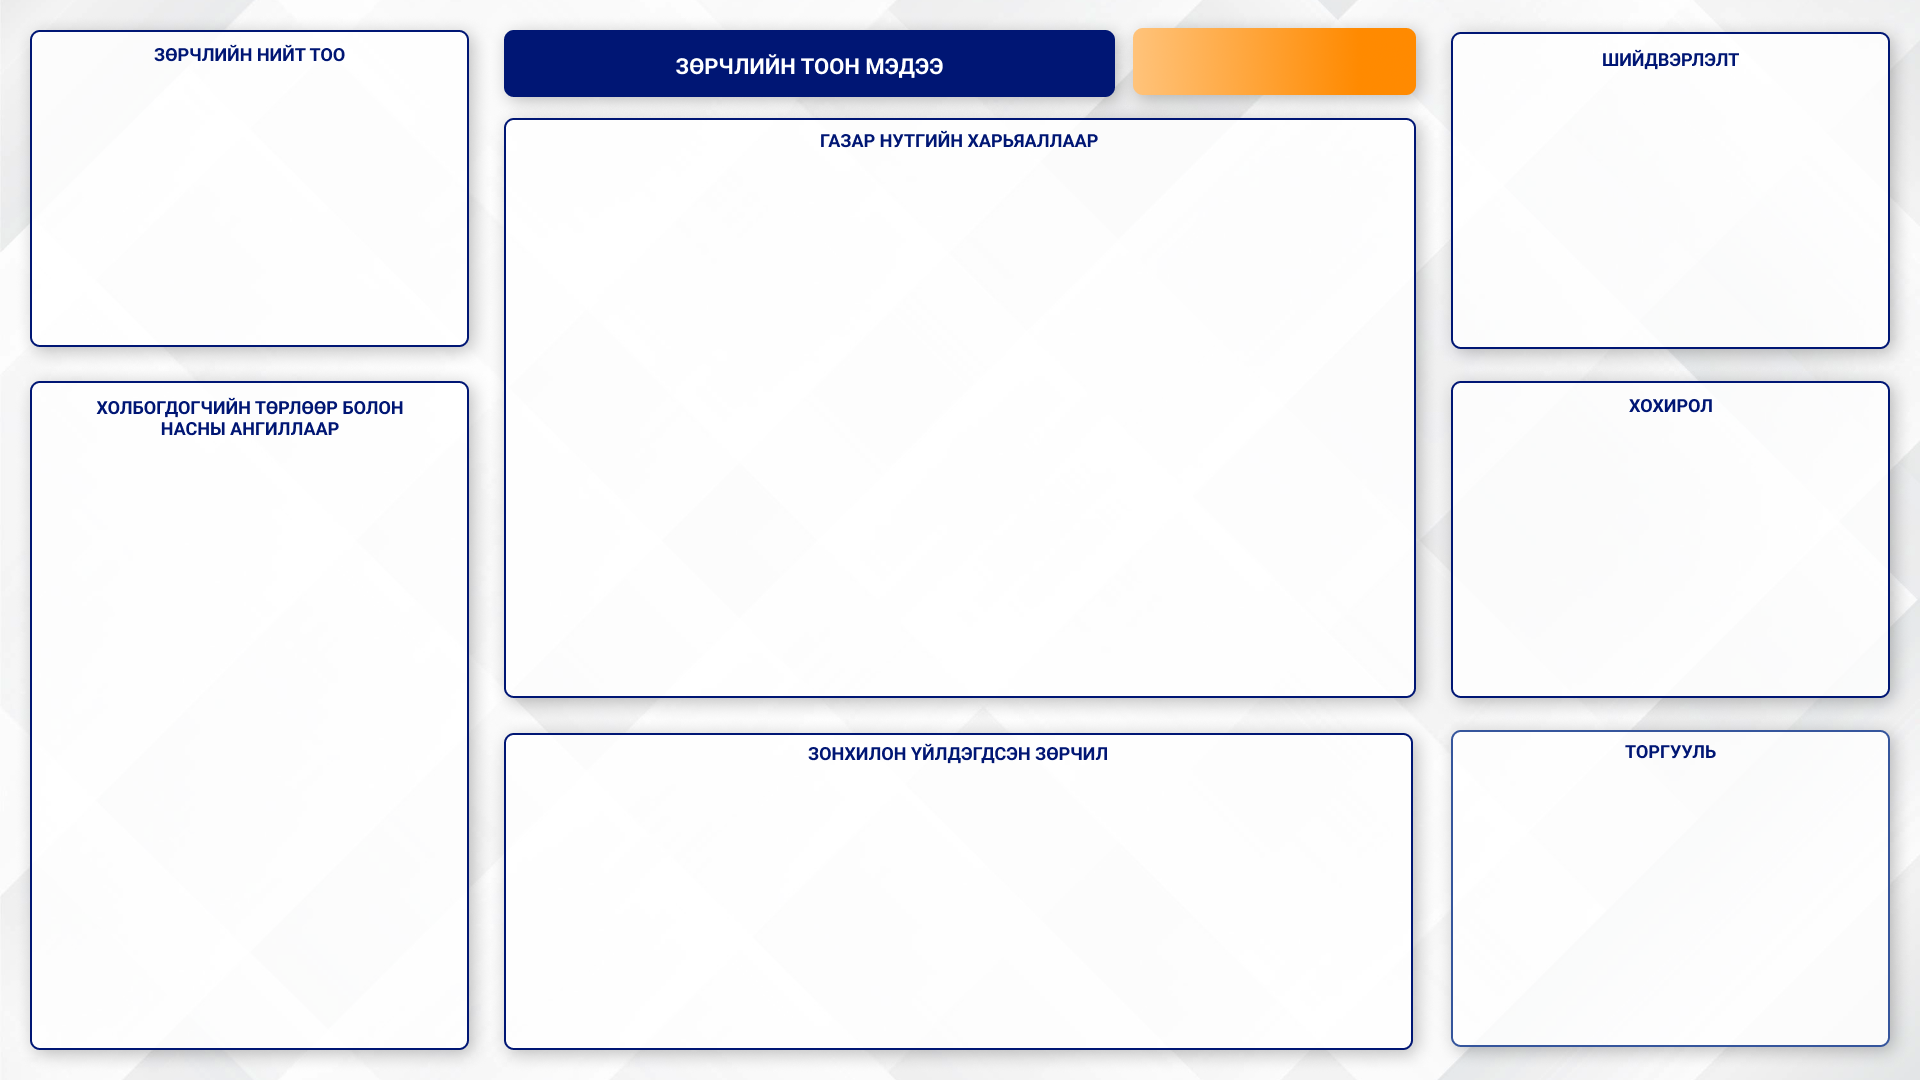
\includegraphics[width=12cm,height=8cm]{images/Frame 10.png}
				\captionof{figure}{Figma дээр гаргасан загвар}
			\end{minipage}
	\item Өрсөн графикуудын харуулж буй тоон утга нь зөв эсэхийг төслийн удирдагчаар хянуулахын үндэсэн дээр бүхий л графикуудын тоон утгыг харуулах Query-уудыг бичсэн. Кодыг хамгийн арын хуудсанд кодын хэсэгт хавсаргасан байгаа.
	\item Том болон жижиг дэлгэцнээс хамааран харуулах шаардлагатай байсан учраас 1366x768 болон 1920x1080 зэрэг хэмжээтэйгээр дашбоардуудыг хийсэн.
  \end{itemize}

  Дээрх алхамууд явагдах явцад хоног тутам хэрэглэгчийн шаардлагад нийцэж байгаа эсэхийг хянуулан тухай бүрт нь нийцүүлэн дашбоардоо сайжруулсаар байсан.
\newpage
Дашбоард: \url{https://public.tableau.com/app/profile/adiya.hella/viz/13x7/1366x768}
\begin{figure}
	\centering
	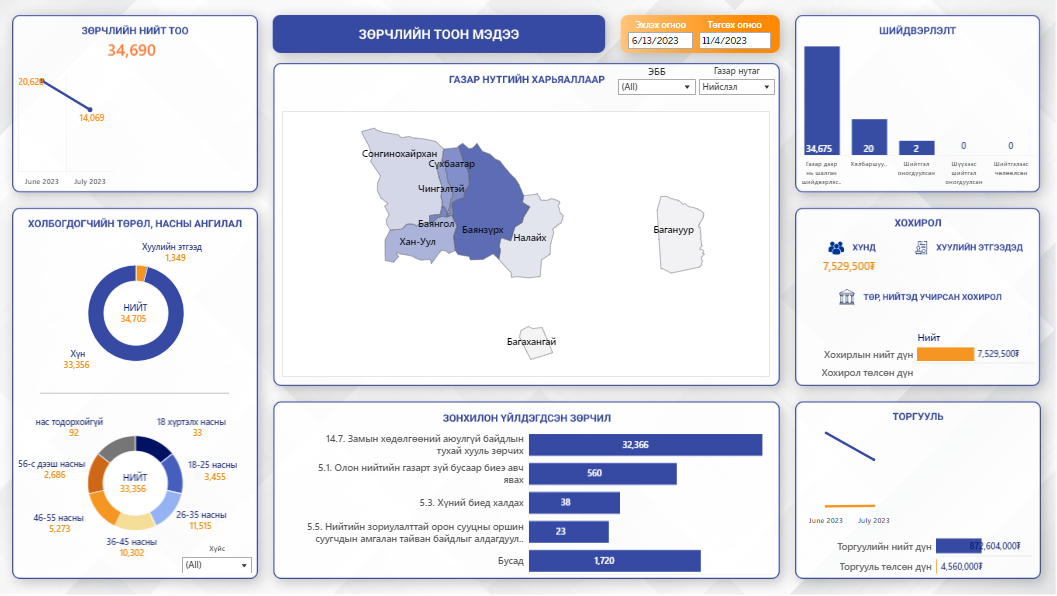
\includegraphics[width=15cm]{images/dash2.PNG}
	\caption{Төслийн явцын дашбоард}
	\label{fig:form}
\end{figure}
